\raggedright

There are two types of DDoS \textbf{attack networks}\textsuperscript{\cite{specht2003taxonomies}}: the \textit{Agent-Handler} model and the \textit{Internet Relay Chat} (IRC) model.

\vspace{0.5cm}

The Agent-Handler model consists of: clients - where the attacker communicates with the rest of the DDoS system, handlers - which are software packages located on the Internet that the clients use to communicate with the agents, and agents - which carry out the attack(s).

The IRC model operates through the use of an online chatting system. It allows multiple parties to connect and message eachother in real time. IRC servers are located throughout the Internet and have public and private channels. Public channels allow multiple users to chat and share content with eachother, and users of that channel can see all other users and messages within the channel. Private channels, however, are setup by individuals to communicate directly with specific users. This protects the names and messages of the users from those who do not have access to the channel.

\vspace{0.5cm}

\begin{figure}[h]
	\begin{subfigure}{0.5\textwidth}
		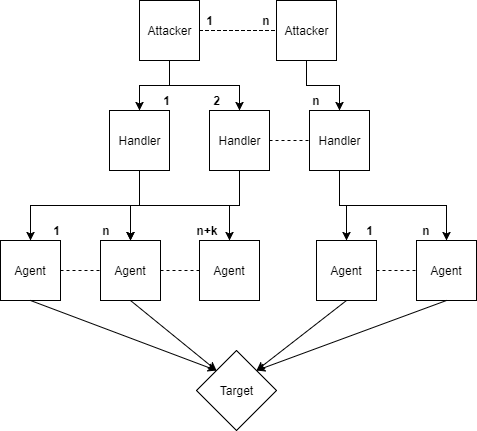
\includegraphics[width=0.9\linewidth, height=7.5cm]{img/ddos_agent_handler_model.png} 
		\caption{Agent-Handler Model}
	\end{subfigure}
	\begin{subfigure}{0.5\textwidth}
		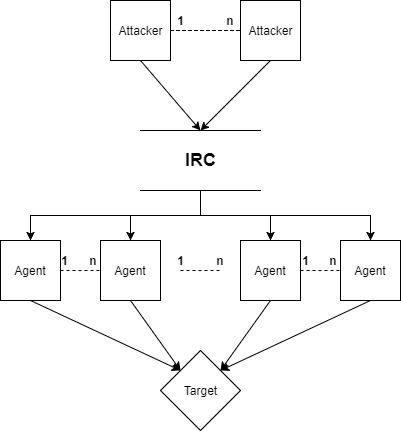
\includegraphics[width=0.9\linewidth, height=7.5cm]{img/ddos_irc_model.png}
		\caption{IRC Model}
	\end{subfigure}
	\caption{Agent-Handler and IRC Models\textsuperscript{\cite{specht2003taxonomies}}}
\end{figure}